%!TEX root = ../dokumentation.tex
\chapter{Selection of Technologies for Prototyping}\label{cha:Technologies}

One of the core aspects of a microservice architecture is the communication \cite[p.~60]{Bruce.2019}.
This includes the inter-microservice communication but also the communication beyond the microservice environment to the client itself.
Especially after the deployment, monitoring systems are crucial for operation, in order to collect metrics and observe the system \cite[p.~313]{Bruce.2019}.
With a preceding research, criteria based on the requirements researched in chapter \ref{cha:Requirement} are used to determine, which technology should be tested through prototypes.

\textbf{Researching Technologies}

In order to select technologies and frameworks for development of prototypes for evaluation, research is needed in both aforementioned aspects of a microservice environment, namely communication and monitoring, to find possible technologies.
Although other aspects, such as testing, project build and deployment, and engines are important, these are deliberately left out due to the timely boundaries of this work.
In the following either practical implementations of protocols or complete frameworks for both aspects are presented briefly.

\section{Communication}\label{cha:Technologies:communication}
%!TEX root = ../../dokumentation.tex

Generally speaking, communication can be done synchronously or asynchronously.
In the context of a microservice architecture, asynchronous communication is highly recommended due to its decoupled and non-blocking nature.
Although such an event based communication is favorable in distributed systems, as in microservices, synchronous messaging may also be used, if a specific behavior in another service is needed \cite[p~.34f]{Hofmann.2016}\cite[p.~89]{Newman.2015}.
Consequently, both forms of service communication need to be analyzed separately.

%!TEX root = ../../dokumentation.tex
\textbf{Synchronous Messaging}

For synchronous messaging, the architectural concept of \ac{REST}, the \ac{RPC} framework \textit{gRPC} and lastly the data query language and runtime \textit{GraphQL} are presented.
Although a lot more alternatives are available, the aforementioned options each represent vastly different concepts.
They are selected as they are the most recent and widespread used technology in their category \cite{Mohilo.2019}\cite{Smith.382018}.
Alternatives to \ac{REST} could be \textit{SOAP} (over \ac{HTTP}) for instance.
Likewise, instead of \textit{gRPC}, implementations such as Java RMI, Apache Thrift or even XML-RPC (precursor to \textit{SOAP}) would be viable options as well \cite{Giro.2019}\cite[p.~62f.]{Bruce.2019}.

\subsection{RESTful HTTP}\label{cha:Technologies:communication:rest}

\acf{REST} is an architectural style which focuses on the concept of resources.
Resources shown externally can be completely decoupled from its internal format.
Furthermore, the resources can be encoded in any arbitrary format, such as \ac{HTML}, \ac{XML} or \ac{JSON} and are accessed through resource methods \cite{Restfulapi.net.23.05.2020}.
A further description of the total 6 guiding principles can be seen in Fieldings work \cite{Fielding.15.03.2002}.
In theory \ac{REST} can be used with any underlying protocol, however, in practice \ac{REST} is commonly used together with \ac{HTTP}, hence the name RESTful \ac{HTTP}.
A widely used and recommended model is the Richardson Maturity Model, which describes resource management, the usage of \ac{HTTP} verbs and hypermedia controls \cite{Fowler.2010}.

With the use of \ac{HTTP}, verbs such as \textit{GET}, \textit{POST}, \textit{DELETE}, single endpoints serving multiple purposes are possible, as seen in Table \ref{tab:restExample}.
Furthermore, support of RESTful communication for proxies, caching services and load balancers as well as security measures is available due to the \ac{HTTP} ecosystem.
On the one hand this fact can make \ac{REST} easy to adopt and to ensure interoperability with preexisting architectures.
On the other hand however, this also leads to the necessity of a secure and scalable communication infrastructure (e.g. use of \ac{TLS} for encryption ) as a base \cite[p.~100]{Newman.2015}.

Another benefit, that RESTful communication provides (if implemented according to the Richardson Maturity Model), is the hypermedia control for resources or \enquote{Hypermedia as the enginge of application state} (HATEOAS).
The concept of hypermedia allows clients to perform interactions with the referenced links, embedded in the response.
As requests are only bound to a reference and not beforehand known direct endpoints, clients are abstracted and the implementation can be changed, as long as the semantic of a response does not change.
Consequently, both client and server implementations are decoupled, as the common denominator is the hypermedia control.
Due to the progressive discovery of the \ac{API} that this hypermedia approach entails, the communication may be more verbose, compared to other technologies.

\begin{table}
	\centering
	\begin{tabular}{ |l|l| }
		\hline
		Action               & REST operation               \\
		\hline
		Get news item        & /news/\{id\} \textbf{GET}    \\
		Get (all) news items & /news/ \textbf{GET}          \\
		Delete news item     & /news/\{id\} \textbf{DELETE} \\
		Update news item     & /news/\{id\} \textbf{PUT}    \\
		Create news item     & /news/\{id\} \textbf{POST}   \\
		\hline
	\end{tabular}
	\caption{Exemplary \ac{REST} operations on news item object} \label{tab:restExample}
\end{table}

\subsection{ gRPC}\label{cha:Technologies:communication:grpc}

Developed in 2015 by Google, \textit{gRPC} is an open source \ac{RPC} system, which uses HTTP2 for transport \cite{gRPCAuthors.25.05.2020}.
As it is an \ac{RPC} framework, characteristics, such as tighter coupling, but on the other hand also high performance messaging apply \cite[p.~93f.]{Newman.2015}.
Likewise server and client code can be generated automatically for a variety of targets.
In the case of \textit{gRPC}, as of May 2020, 11 languages are officially supported, namely \textit{C/C++, C\#, Dart, Go, Java, Kotlin, Node.js, Objective-C, PHP, Python, Ruby}.

Unlike \ac{REST}, \textit{gRPC} relies on an \ac{IDL} to define the services, which per default are \textit{protocol buffers} (often abbreviated as \enquote{protobuf})
Apart from using protocol buffers as its \ac{IDL}, \textit{gRPC} can also use it as its message interchange format.
In order for \textit{gRPC} to be able to serialize structured data, each data type may be described in a \textit{*.proto} file, although other similar and popular \acp{IDL}, such as Apache Thrift, as well as \ac{JSON} or \ac{XML} are supported \cite{gRPCAuthors.25.05.2020b}\cite{gRPCAuthors.25.05.2020d}. \\

\begin{lstlisting}[caption=Example of data structure in a \textit{*.proto} file, label=listing:protobufdata]
message Studienarbeit {
string title = 1;
int32 id = 2;
bool passed = 3;
}
\end{lstlisting}

\begin{lstlisting}[caption=Example of service definition in a \textit{*.proto} file, label=listing:protobufservice]
service Greeter {
// Sends a greeting
rpc SayHello (HelloRequest) returns (HelloReply) {}
}

// The request message containing the user's name.
message HelloRequest {
string name = 1;
}

// The response message containing the greetings
message HelloReply {
string message = 1;
}
\end{lstlisting}

An example of such a data object description, using a protocol buffer definition can be seen in Listing \ref{listing:protobufdata}.
With a proto file, according stubs can be generated for target programming languages, by using the protocol buffer compiler \textit{protoc}.
Services to be used can be defined in \textit{gRPC} as well, as seen in Listing \ref{listing:protobufservice} \cite{gRPCAuthors.25.05.2020b}\cite{gRPCAuthors.25.05.2020c}.
The code generated by \textit{protoc} in according target languages can then be used in server and clients as depicted in Figure \ref{img:grpcoverview} \cite{gRPCAuthors.25.05.2020b}.

\begin{figure}[hb]
	\centering
	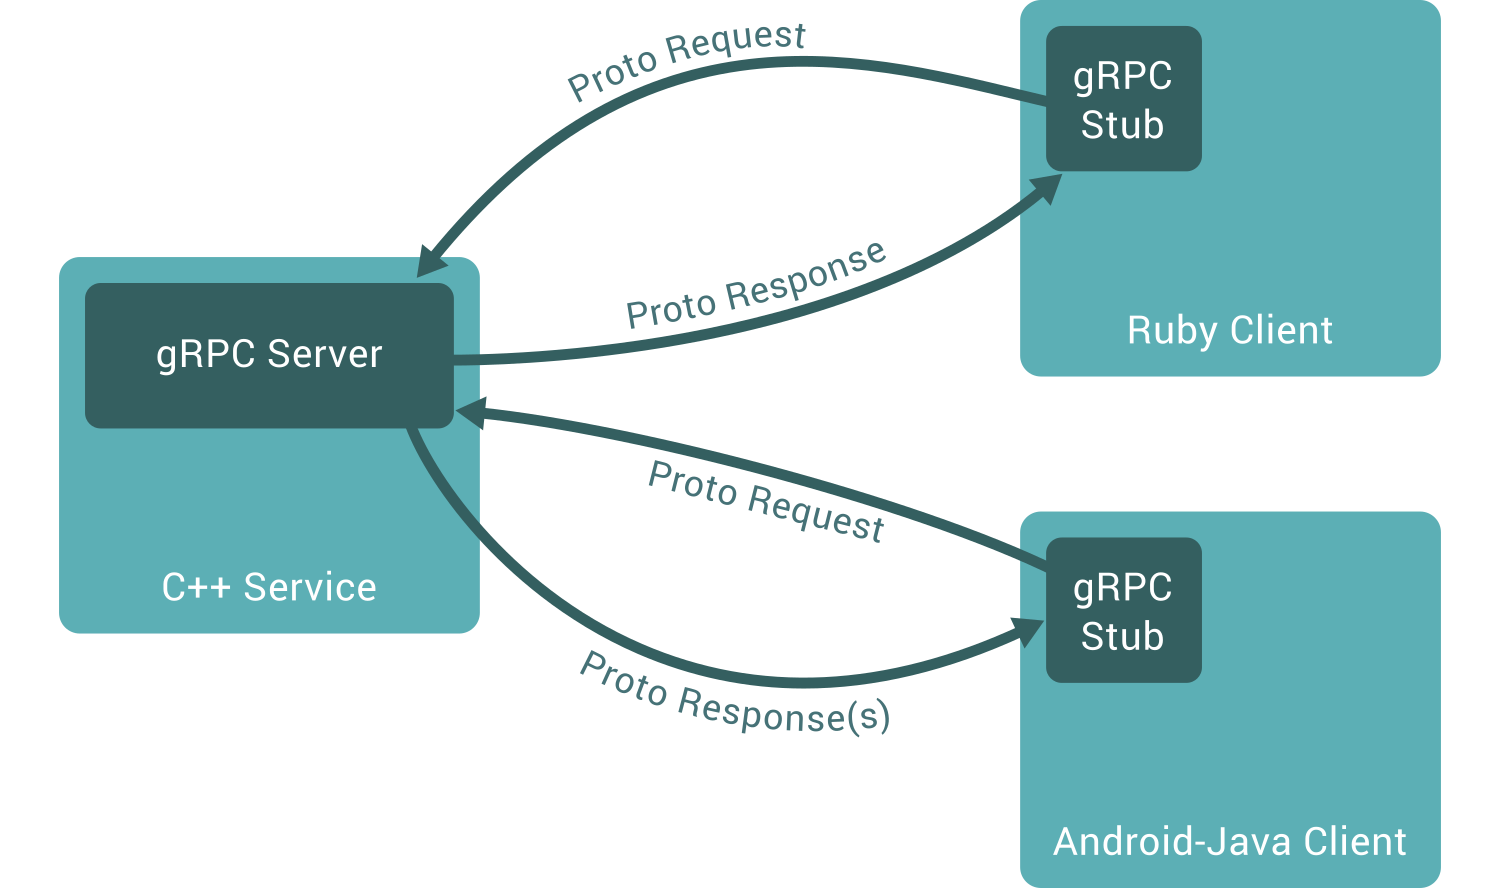
\includegraphics[width=\textwidth, height=0.25\textheight, keepaspectratio]{gRPCoverview.png}
	\caption{gRPC polyglot implementation overview}
	\label{img:grpcoverview}
\end{figure}

A common use case for \textit{gRPC} currently is the inter service communication in microservices, especially, where strict specification and low latency actions need to be executed \cite{Sturgeon.2016}.
The concept of \textit{gRPC} is based around an API contract and strict semantics.
Protocol buffer as a small binary format has a faster serialization (\enquote{de-/marshalling}) and is more efficient, in contrast to the human readable \ac{JSON} used in RESTful \ac{HTTP} applications.
This makes \textit{gRPC} especially useful for network constrained environments and high throughput communication.
As protocol buffer serves as an \ac{IDL}, \textit{gRPC} user have to follow a prescriptive formal specification, as opposed to loose models and implementation levels (e.g. Richardson Maturity Model) \cite{NewtonKing.2019}.

Furthermore, due to the use of HTTP2, \textit{gRPC} supports bi directional streaming, making point-to-point real time communication possible.
Consequently, the need for polling or switching protocols to \textit{WebSocket} for instance can be eliminated.
Other supported forms of streaming are server to client, client to server and unary.

In contrast to \ac{REST}, the usage of \textit{gRPC} in the browser is limited and not supported by default.
Consequently extensions like \textit{gRPC-Web} are needed, which includes an \textit{gRPC} proxy and a JavaScript client for the browser.
Furthermore, \textit{gRPC} messages can not be broadcasted and are not human readable due to protocol buffers being a binary format.
Nonetheless \textit{gRPC} represents a well supported \ac{RPC} communication framework, which is beneficial for efficient inter process communication in distributed client server architectures.
Especially in the context of polyglot microservice environments, the streaming capabilities and low latency of \textit{gRPC} are useful, not only for backend communication but also for applications on (mobile) clients \cite{NewtonKing.2019}\cite{1&1IONOSSE.2020}.

\subsection{GraphQL}\label{cha:Technologies:communication:graphql}

\textit{GraphQL} can be defined as both a data query language as well as a runtime.
The language is used for writing requests for client applications and is close to
\ac{JSON} (as seen in Listing \ref{listing:graphqlquery}).
Contrary to that, the \textit{GraphQL} runtime layer is needed on the server, in order to transform requests into existing logic to fetch data \cite[p.7~f.]{Buna.2016}.
The runtime layer is also responsible for accumulation of different data sources (e.g. composite design pattern seen in Figure \ref{img:compositedesigngraphql})
Although the service is transport agnostic, the most common combination is with \ac{HTTP}.
Furthermore, \textit{GraphQL} has a widespread implementation available similar to \textit{gRPC}, namely \textit{C\# / .NET, Clojure, Elixir, Erlang, Go, Groovy, Java, JavaScript, Julia, Kotlin, Perl, PHP, Python, R, Ruby, Rust, Scala, Swift, OCaml / Reason} \cite{TheGraphQLFoundation.27.05.2020}.

\begin{figure}
	\centering
	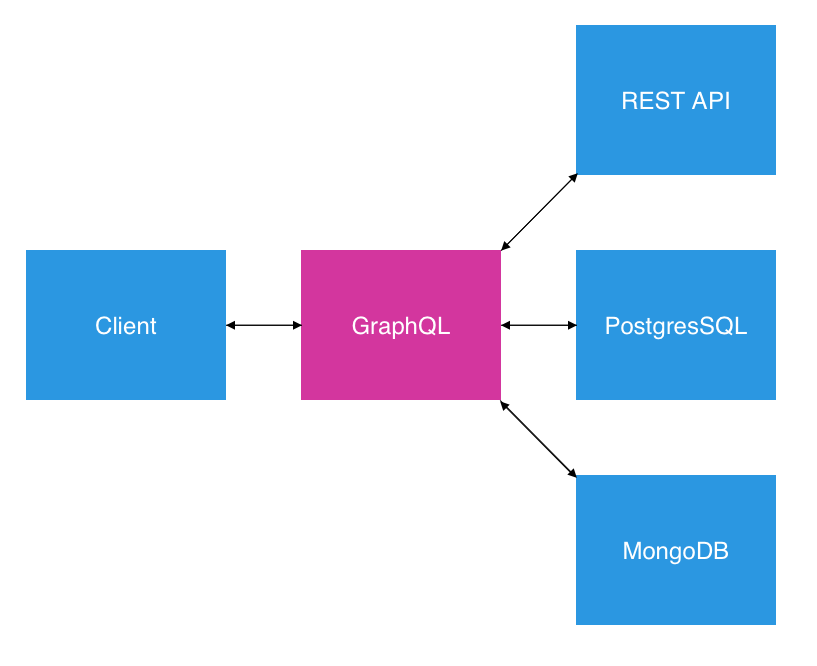
\includegraphics[width=\textwidth, height=0.32\textheight, keepaspectratio]{compositedesigngraphql.png}
	\caption{Composite design pattern in \textit{GraphQL} \cite{Lombard.2018}}
	\label{img:compositedesigngraphql}
\end{figure}

With \textit{GraphQL}, the client specifies the data requirements and only requests the data they need, hence often being referred to as an declarative data fetching language \cite[p.~6f.]{Buna.2016}.
In Listing \ref{listing:graphqlquery} two queries are described, with the according responses seen in Listing \ref{listing:graphqlresponse}.
With the second query, the main characteristics of \textit{GraphQL} are visible \cite[p.~16]{Porcello.2018}:

The data that is served is strongly typed in the \textit{GraphQL} scheme, which makes misuse detection easier \cite[p.~65]{Buna.2016}.
Each data point has a specific type, the scheme \textit{person} has to exist, with predefined field types, such as \textit{filmConnection} as a \textit{PersonFilmsConnection}.
Furthermore \textit{GraphQL} is product centric, which means that it is focused on the clients data needs and the supporting language and runtime.
This also allows for client-specified queries; servers have to provide the capabilities that clients are allowed to consume.
The field \textit{filmConnection} as well as the schemes for the object \textit{films} therefore have to exist.

In cases where the client does not know about the server's type system, the client has to be able to query the scheme with the \textit{GraphQL} language (\textit{Introspection}).
Lastly, every \textit{GraphQL} query can be hierarchical.
Fields can be nested in other fields, as seen with \textit{films} via the \textit{filmConnection}, and the corresponding response is shaped exactly the same \cite[p.~12ff.]{Porcello.2018}\cite[p.~10ff.]{Buna.2016}.

\begin{lstlisting}[caption=Example of GraphQL queries, label=listing:graphqlquery]
// first query
query{
person(personID>5) {
name,
birthYear
}
}
// second query with more fields
query{
person(personID>5) {
name,
birthYear,
filmConnection {
films {
title
}}}
}
\end{lstlisting}

\begin{lstlisting}[caption=Example of GraphQL responses, label=listing:graphqlresponse]
// response to the first query
{
"data": {
"person": {
"name": "Leia Organa",
"birthYear": "19BBY",
}}
}

// response to the second query
{
"data": {
"person": {
"name": "Leia Organa",
"birthYear": "19BBY",
"filmConnection": {
"films": [
{"title":"A New Hope"},
{"title":"The Empire Strikes Back"},
{"title":"The Force Awakens"},
]
}}}
}
\end{lstlisting}

Further exact description about the query language and the scheme as well as the configuration of the runtime are left out in this work, as they are not required for an overview here.

\textit{GraphQL} currently is mostly recommended for Data \acp{API}, especially when the requested data is graph-like.
Similar to \textit{gRPC}, the efficiency through direct querying and low latency, due to the most minimal response size, make \textit{GraphQL} especially useful for applications with a restricted bandwith (e.g. mobile appliances).
RESTful \ac{API} in contrast, may suffer from over- and/or underfetching \cite[p.~3]{Doerrfeld.2018}.

Overfetching occurs when more data is given than actually needed, which may happen especially with large data endpoints with HATEOAS implemented.
On the other hand, when needed data is undercut, the client would have to make multiple requests.
Especially on resource restricted devices, multiple round trips for a single view are inefficient \cite[p.~12f.]{Buna.2016}\cite[p.~24ff.]{Porcello.2018}.
This issue is mitigated in \textit{GraphQL}, as the response is uniform with the request itself.
Moreover, nesting reduces the load on the target device.
In a RESTful API, in order to receive the data of the second request depicted in Listing \ref{listing:graphqlquery}, one would request the \textit{films} of a \textit{person} and receive \textit{filmCollection}, a list of links.
Following that, each link would have to be requested and the field \textit{title} extracted.

\begin{figure}[h]
	\centering
	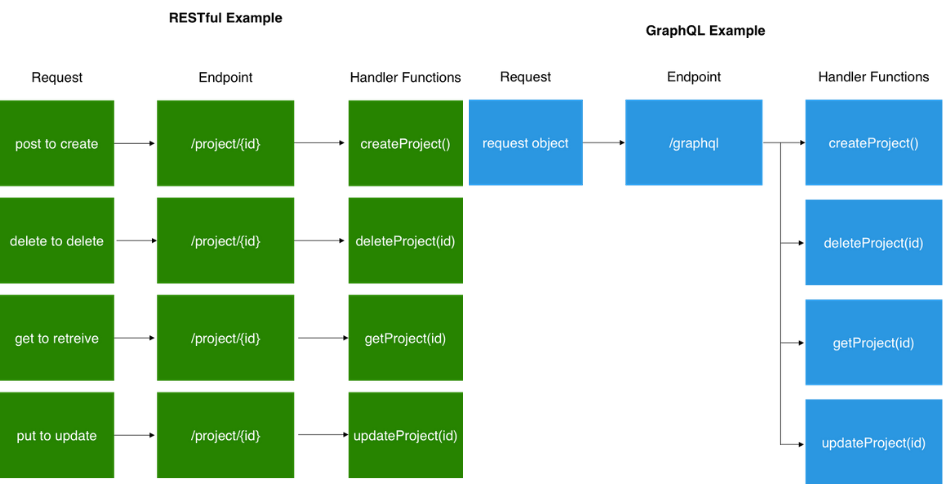
\includegraphics[width=\textwidth, height=0.9\textheight, keepaspectratio]{multiplerestVSgraphql.png}
	\caption{Multiple REST requests vs a single GraphQL request \cite{Lombard.2018}}
	\label{img:restvsgraphqlrequest}
\end{figure}

Furthermore \textit{GraphQL} is easier to scale and maintain due to stronger typing and schema discovery.
Although RESTful \ac{API} implements this with HATEOAS, versioning of endpoints or managing endpoints in general can be cumbersome.
With \textit{gRPC}, flexibility is very limited as it is an \ac{RPC} framework in its nature.
\textit{GraphQL} instead resolves this, by having only one endpoint, with which balancing, orchestration of data sources and version control is possible. (cf. Figure \ref{img:restvsgraphqlrequest})
Consequently, \textit{GraphQL} is the most flexible and scalable when comparing against \textit{gRPC} or a RESTful \ac{HTTP} \ac{API} \cite[p.~29]{Porcello.2018}\cite[p.~11]{Buna.2016}.

Nonetheless, \textit{GraphQL} can be at a disadvantage due to incompatibility with common caching solutions and query complexity.
Each query still needs to be resolved with the target data source, where bottlenecks naturally occur.
This issue especially prevails in situations with a high query depth or query complexity.
Furthermore, rate limiting as typically applied in RESTful \acp{API} are more difficult to apply, because the query depth and complexity weighing can vary a lot \cite{Wieruch.2018}\cite{AltexSoft.2019}.
In most cases, however, \textit{GraphQL} is used as an intermediary, where a \textit{GraphQL} \ac{API} is exposed, but the runtime itself communicates over existing \ac{REST} \acp{API}.
This hybrid proxy variant allows easy adoption and a incremental adoption of \textit{GraphQL} \cite[p.~29]{Porcello.2018}.
\label{cha:Technologies:communication:synchronous}
\clearpage
%!TEX root = ../../dokumentation.tex

\textbf{Asynchronous Messaging}

For asynchronous messaging, the technologies RabbitMQ with its supported protocols, \ac{NATS} and Apache Kafka are presented.
RabbitMQ is used as a representative for all technologies that implement \acf{AMQP}, \acf{MQTT} or \acf{STOMP}.
Apache Kafka is a relatively new technology that has attracted much attention.
It was already introduced in the TechnologyRadar in 2016 \cite{ThoughtWorks.01.06.2020} and a new technique \textit{Event streaming as the source of truth} is becoming more and more popular \cite{ThoughtWorks.01.06.2020b}, which fits perfectly with Apache Kafka.
\ac{NATS} is also quite new, but its main focus is on availability, while RabbitMQ and Apache Kafka focus more on consistency.
Therefore, these three technologies represent a wide range of asynchronous messaging systems.

\subsection{RabbitMQ}\label{cha:Technologies:communication:rabbitmq}

RabbitMQ is an implementation of the \acf{AMQP}.
The protocol follows a Publish-Subscribe pattern.
The communication flow of \ac{AMQP} is shown in Figure \ref{img:rabbitmqamqp}.
It is important to note that multiple publishers can publish to the same exchange entity, one exchange entity can route to multiple queues and multiple consumer can listen at one queue.
The routing of an exchange entity can be configured in four different ways.
To explain the different configurations, it is important to note that each message contains a routing key and can contain n-header information.
Both are used by the exchange entities, but in different ways depending on the configuration.
The following list shows the differences between the configurations in terms of how they route a message to an associated queue \cite{RabbitMQ.2020}\cite[p.~26ff.]{SanjayAiyagarietal.2008}.

\begin{itemize}
	\item Direct: (default) Route a message based on its routing key.
	\item Fanout: Copies the message and sends it to each queue, regardless of the message information.
	\item Topic: Works like Fanout, but also uses the routing key. Queues define regular expressions to determine whether a routing key can be associated with that queue.
	\item Header: Ignores the routing key and uses header information to route a message. This is highly configurable by itself.
\end{itemize}

Exchange entities and queues can be defined in advance or by the publisher and consumer.
If they are defined by the publisher or consumer, the required configuration is provided and sent to RabbitMQ.
When connecting to an exchange or queue its configuration must be provided.
If it doesn't exist, then a new one is created.
If it does exist and the configuration matches the existing one, then a connection is established.
If the provided configuration does not match the configuration of the existing exchange or queue, an error is thrown.
Publisher define exchanges and consumer define queues.
When defining a queue, a binding is required that connects the queue to an exchange entity.
The binding can consist of a routing key (direct exchange), regular expression (topic exchange) or nothing (fanout exchange and header exchange) \cite{RabbitMQ.2020}.

It is important to add that RabbitMQ mostly follows the \ac{AMQP} specification, but small adjustments for usability and functionality extensions were made \cite{RabbitMQ.2020b}.
Also, \ac{AMQP} is not the only standard protocol supported by RabbitMQ.
The protocols \ac{STOMP} and \ac{MQTT} are supported via a plugin as well \cite{RabbitMQ.27.05.2020}.

\begin{figure}
	\centering
	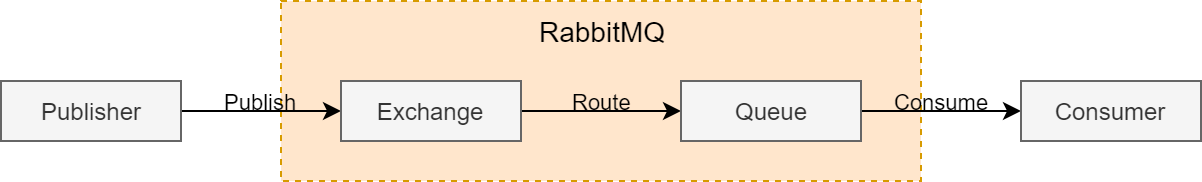
\includegraphics[width=\textwidth, height=0.9\textheight, keepaspectratio]{RabbitMQ_AMQP.png}
	\caption{RabbitMQ communication flow}
	\label{img:rabbitmqamqp}
\end{figure}

\paragraph{STOMP plugin}

As the name suggests, \acf{STOMP} is a simple protocol where messages are sent in frames.
A frame is a text message consisting of a command, an optional header and an optional body.
\ac{STOMP} requires a underlying 2-way streaming network protocol to send frames between client and server.
The communication flow is shown in Figure ~\ref{img:rabbitmqstomp}.
A client can be either a consumer or a publisher.
In both cases, the client only needs to know the connection information of the server for setup.
Unlike \ac{AMQP}, where the client also defines exchanges and queues, \ac{STOMP} requires that the logic is defined in the server.
The clients cannot define the routing behavior of the server, so the server must provide this logic.
To route a message, the server can use anything within it \cite{.25.09.2015}.
The RabbitMQ implementation of \ac{STOMP} has several routing options and each is provided by a separate destination.
To send a message to a specific destination, a \textit{destination string} can be used \cite[p. 191]{Roy.2018}.

\begin{figure}
	\centering
	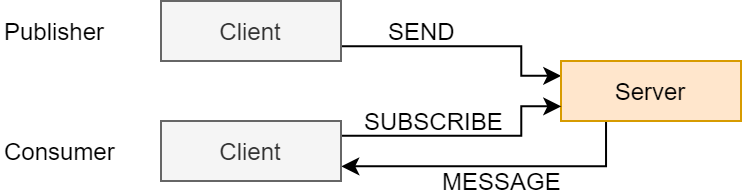
\includegraphics[width=\textwidth, height=0.9\textheight, keepaspectratio]{RabbitMQ_STOMP.png}
	\caption{RabbitMQ communication flow using STOMP}
	\label{img:rabbitmqstomp}
\end{figure}

\paragraph{MQTT plugin}

\ac{MQTT} is located between \ac{STOMP} and \ac{AMQP} from a functionality point of view.
It provides a basic routing like the \ac{AMQP} topic exchange shown in Figure ~\ref{img:rabbitmqmqtt}.
A client can publish a message on a topic (shown in Figure ~\ref{img:rabbitmqmqtt} with topic \textit{cat1/top1} and \textit{cat1/top2}).
A client can also subscribe to topics.
This is shown in Figure \ref{img:rabbitmqmqtt}, where \textit{Subscriber B} subscribes to both topics and therefore receives messages from both topics.
As with \ac{AMQP} topic exchange, the messages are copied and sent to each subscriber \cite[p.~4ff.]{Hillar.2017}\cite{AndrewBanks.2014}.
Finally, each message contains a \acf{QoS} attribute that determines how the message is handled in case of errors \cite{AndrewBanks.2014}.

\begin{figure}
	\centering
	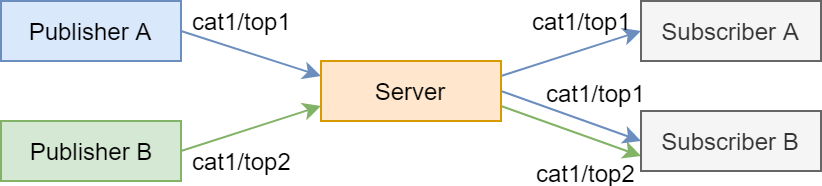
\includegraphics[width=\textwidth, height=0.9\textheight, keepaspectratio]{RabbitMQ_MQTT.png}
	\caption{RabbitMQ communication flow using MQTT}
	\label{img:rabbitmqmqtt}
\end{figure}

\paragraph{Protocol selection}

RabbitMQ can be used in several ways because it supports three protocols.
Consequently, the question remains which protocol to use.
In general, it is advisable to use a protocol that is already supported by an environment.
Another point to consider are the required communication features.
\ac{AMQP} is feature-rich, which can be too complicated for some application environments.
It also has a high latency, which can be a problem for unreliable networking of mobile devices \cite[p. 177]{Roy.2018}.
As described above, \ac{MQTT} has fewer features than \ac{AMQP} and \ac{STOMP} is even more lightweight than \ac{MQTT} \cite[p. 189]{Roy.2018}.
When deciding which protocol to use, it is also helpful to consider other projects.
For example, \ac{MQTT} is often used for \ac{IoT} applications.
This is probably due to the small code footprint or its suitability for low-bandwidth environments \cite[p. 178]{Roy.2018}\cite{AndrewBanks.2014}.
When using \ac{STOMP} the big advantage is that messages are sent in human-readable form (text based), but this is also a disadvantage.
\ac{AMQP} and \ac{MQTT} are binary and therefore more efficient than \ac{STOMP} in transmitting data.
Finally, it is important to mention that the \ac{STOMP} plugin for RabbitMQ adds an overhead, because RabbitMQ uses proxied \ac{AMQP} connections to communicate the translated \ac{STOMP} data \cite[p. 200]{Roy.2018}.

\paragraph{Conclusion}

RabbitMQ is very flexible because it supports several standard protocols, allowing for future technology exchanges.
Which protocol should be used depends on many factors, as described above.
Finally, some important factors that support RabbitMQ for the election, based of the persona needs.

RabbitMQ keeps messages in \ac{RAM} if possible and only when the \ac{RAM} is full, the messages are moved into memory.
To ensure good performance, additional nodes can be added to a running cluster, allowing dynamic scaling.
To ensure availability, nodes can be replicated and the message acknowledgment provides a delivery guarantee.
Another easy to implement feature in RabbitMQ is \textit{multicast}, which can be achieved via a fanout exchange \cite[p.~230ff.]{Dobbelaere.2017}.

\subsection{NATS}\label{cha:Technologies:communication:nats}

The \acf{NATS} is a communication technology that follows the \textit{publish-subscribe} pattern.
Its core objectives are simplicity, performance, and reliability \cite[p.~8]{Quevedo.2018}.
Communication is session-based and a session starts and ends with a connection.
When a session is closed, no data is persisted \cite[p.~3]{Quevedo.2018}.
\ac{NATS} is a non-binary transmission and only provides an \textit{at-most-once} \ac{QoS} when transmitting data \cite[p.~20]{Quevedo.2018}.
There is another popular project called \textit{NATS Streaming}, which adds an abstraction layer over \ac{NATS} and provides an \textit{at-least-once} \ac{QoS} \cite[p.~10f.]{Quevedo.2018}.
It also does not persist or buffer information by default, making it a true \textit{fire and forget} system \cite[p.~8]{Quevedo.2018}.

\ac{NATS} supports the subscription models \textit{fan-out} and \textit{queue subscription}.
Fan-out is the default, and it works like the \ac{AMQP} fanout exchange, but it still uses the subject (or topic in the \ac{AMQP} context).
So, any client that subscribes to a subject will receive all messages in that subject \cite[p.~6]{Quevedo.2018}.
Subjects can be divided into namespaces with a "." (\textit{period}).
A Subscription can be more general by using wildcards, such as "*" (\textit{asterisk}) for partial or token match and ">" (\textit{greater}) for full wildcard \cite[p.~31]{Quevedo.2018}.
Figure \ref{img:natspubsub} shows an example of fan-out communication with multiple clients and namespaces:
\textit{Client C} only receives the message from \textit{Client A}, because it has subscribed the topic \textit{data.test}, whereas \textit{Client D} receives every message published to a subject which starts with the namespace \textit{data}.
Therefore, it receives both messages.

\begin{figure}
	\centering
	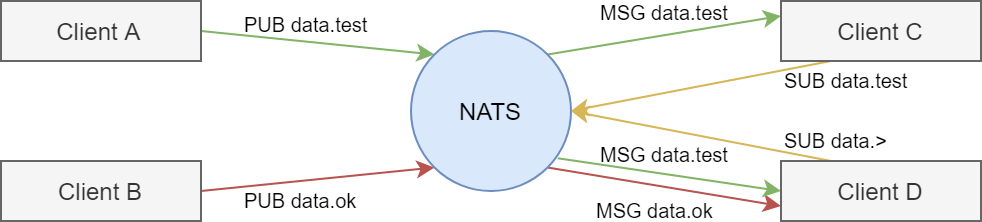
\includegraphics[width=\textwidth, height=0.9\textheight, keepaspectratio]{NATS_Fanout.png}
	\caption{NATS publish subscribe example}
	\label{img:natspubsub}
\end{figure}

The other subscription model \textit{queue subscription} works like \ac{AMQP} \textit{direct exchange}.
When a message is published to a subject, it is distributed to only one subscriber, instead of all.
The two subscription modes can be combined \cite[p.~34ff.]{Quevedo.2018}.
For example, a subject has two clients (\textit{A} and \textit{B}), which are subscribed via a \textit{queue subscription} and one client (\textit{C}) via a \textit{fan-out}.
Then clients \textit{A} and \textit{B} receive messages alternately and \textit{C} receives each message.

A powerful technique of \ac{NATS} is the \textit{request-response} pattern, which enables a completely asynchronous implementation.
An example is shown in Figure \ref{img:natsreqres}, where \textit{Client B} sends a request and \textit{Client A} responds.
This can be archived when \textit{Client B} provides a response subject and its name is passed along with the request.
So, \textit{Client A} knows where to publish the response \cite[p.~38ff.]{Quevedo.2018}.

The Request-Response pattern can be further improved if necessary, by reducing the latency.
To achieve this, \textit{Client A} must be replicated and \textit{Client B} must unsubscribe the response subject, once a message has been retrieved.
It is important that \textit{Client A} and its replicas use the \textit{fan-out} subscription model and the response subject should be unique to avoid collisions.
The result of this approach is that many responses are wasted because only the fastest respond is used.
However, if the main concern is time, this technique allows even faster responses.
Therefore it is called \textit{Lowest Latency Response} \cite[p.~40f.]{Quevedo.2018}.

\begin{figure}
	\centering
	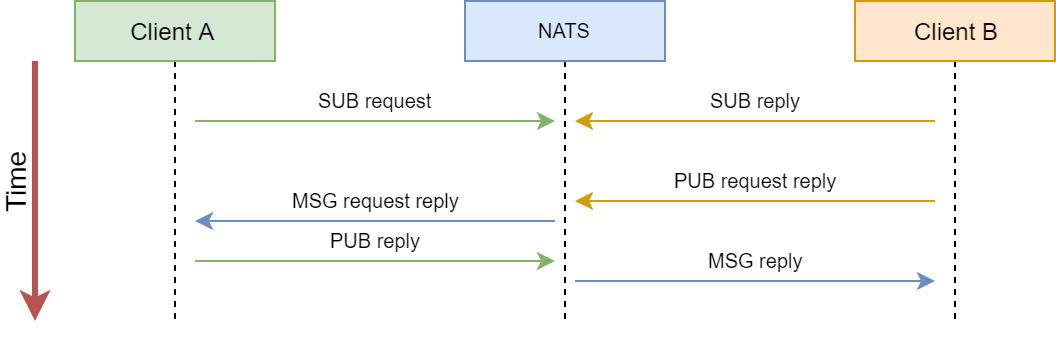
\includegraphics[width=\textwidth, height=0.9\textheight, keepaspectratio]{NATS_request_response.png}
	\caption{NATS request response example}
	\label{img:natsreqres}
\end{figure}

After considering the functionality of \ac{NATS}, the next step is to evaluate it based on the requirements of the personas.
One of the core objectives of \ac{NATS} is performance \cite[p.~8]{Quevedo.2018} and this is illustrated in a benchmark.
For example, in a benchmark comparison between \textit{NATS Streaming} and \textit{Apache Kafka}, \textit{NATS Streaming} was faster in almost every test \cite{TylerTreat.2016}.
It is important to note that \textit{NATS Streaming} uses \ac{NATS} in the core and adds an abstraction layer above it.
This indicates that \ac{NATS} is even faster than shown in the benchmark.
Another important factor is scalability and \ac{NATS} provides a high availability support via a clustering mode that is set up as a full-mesh of servers \cite[p.~8]{Quevedo.2018}.
Another key objective is simplicity \cite[p.~8]{Quevedo.2018}, which is represented by the relatively simple command set.
However, these allow powerful combinations such as mixing of subscription modes \cite[p.~35f.]{Quevedo.2018} and the \textit{Lowest Latency Response} technique \cite[p.~40f.]{Quevedo.2018}.
An important factor to consider is that \ac{NATS} core provides the \textit{at-most-once} \ac{QoS}.
This can be extended to \textit{at-least-once} using the \textit{NATS Streaming} project \cite[p.~10f.]{Quevedo.2018}.
After all, \ac{NATS} tries to stay alive at all costs.
This means that in case of a client connection that accumulates too much data without emptying it, the \ac{NATS} server will disconnect from the client to protect itself \cite[p.~9]{Quevedo.2018}.

\subsection{Apache Kafka}\label{cha:Technologies:communication:kafka}

Apache Kafka (in the following only \textit{Kafka}) is a log-based distributed streaming platform and offers high availability, storage and linear scale-out \cite[p.~14]{Stopford.2018}.
For fault tolerance and linear scale-out, the data is distributed across many machines \cite[p.~17f.]{Stopford.2018}.
\textit{Kafka} is suitable for a variety of applications, but before describing them, it is important to explain how \textit{Kafka} works.

Like the other asynchronous communication technologies, \textit{Kafka} follows the \textit{publish-subscribe} pattern.
This means that a client can publish a message to a topic, and a subscribed consumer receives the message.
In \textit{Kafka}, a message is treated like a log, which means that it is immutable and added to a message log.
The topics are divided into partitions \cite[p.~30]{Kumar.2017}, and each partition has its own message log \cite[p.~33]{Kumar.2017}.
To determine which message is routed to which partition, the message key is used \cite[p.~41]{Kumar.2017}.
To ensure high availability, topic partitions are replicated, where one partition is the leading partition and the others are the following partitions.
If the leader fails, a new leader is selected from the followers \cite[p.~33]{Kumar.2017}.

Partitions and their replicas are distributed among several brokers \cite[p.~17]{Stopford.2018}, and a broker can only have one or two partitions of the same topic.
A \textit{Kafka} cluster consists of several nodes, which in turn have several brokers \cite[p.~27]{Kumar.2017}.
This combination allows \textit{Kafka} to scale particularly well, so that it is no problem to have 100 nodes or even more \cite[p.~20]{Stopford.2018}.

The next important part of \textit{Kafka} is \textit{Zookeeper}.
It is responsible for several tasks, and without it \textit{Kafka} would not work.
For example, \textit{Zookeeper} takes care of the broker states, because broker do not persist their state \cite[p.~27]{Kumar.2017}\cite[p.~37f.]{Kumar.2017}.
\textit{Zookeeper} also knows the distributed locations of the partition leaders and followers \cite[p.~34]{Kumar.2017}.

A client who sends messages to a topic is called a producer, and a client who receives messages is called a consumer.
Each consumer belongs to a consumer group, and a consumer group can consist of several consumers \cite[p.~36f.]{Kumar.2017}.
Within a consumer group, only one consumer can be assigned to a topic partition.
This limits the degree of parallelism in a single consumer group \cite[p.~30f]{Kumar.2017}.
To publish or subscribe to a topic, the publishers or consumer needs to know which topic partition is relevant for them.
This means that a message is published or consumed directly from a topic partition, rather than from a topic.
Publishing or consuming a message is only possible from a topic partition leader \cite[p.~33]{Kumar.2017}\cite[p.~36]{Kumar.2017}.

All the parts described are combined in the Figure \ref{img:kafkacomflow}, where an example communication is shown.
The actual message transmission is only a small part, and a lot of work is done beside it.
In addition, the described communication flow shows the standard behavior, which can be changed.

Before any communication can take place, \textit{Zookeeper} must collect information about the locations of the topic partition (\textit{1}).
This information is then distributed to the producers and consumers (\textit{2}).
Now the producer knows the destination for the message and sends it to the lead partition \textit{A} (\textit{3}).
Partition \textit{A} stores the message and then informs \textit{Zookeeper} and the publisher about the successful writing (\textit{4}).
\textit{Zookeeper} then informs the consumer about a new message that is available (\textit{5}).
Now consumer \textit{A} can read the new message (\textit{6}) and updates its state at \textit{Zookeeper} (\textit{7}).

\begin{figure}
	\centering
	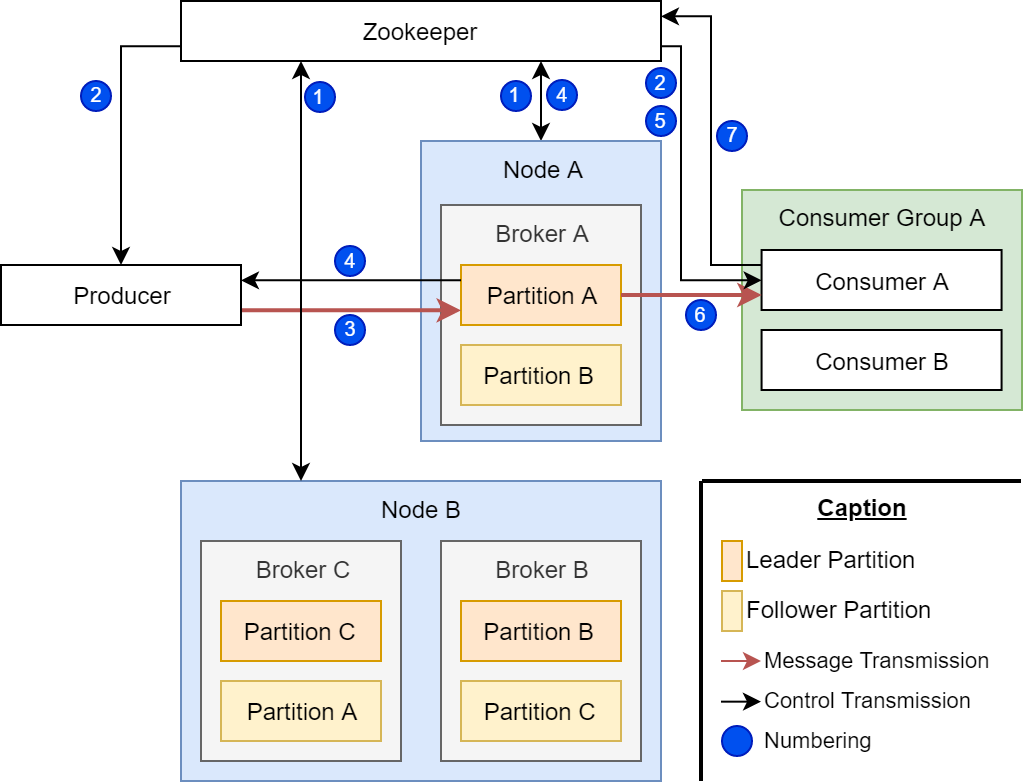
\includegraphics[width=\textwidth, height=0.9\textheight, keepaspectratio]{kafka_communication_flow.png}
	\caption{Kafka communication flow}
	\label{img:kafkacomflow}
\end{figure}

The last important part to complete \textit{Kafka}'s explanation is the message log within a partition.
Publishing a message to a message log within a partition involves several steps.
The process is shown in Figure \ref{img:kafkapubmsg}.
After a leading partition receives a message, it calculates the message offset, which is the identifier of a message within a partition.
The message is then appended to the message log, but not committed \cite[p.~18]{Stopford.2018}.
In addition, the message is sent to all its partition followers.
Each follower partition replies with an acknowledgment, and once everyone has responded, the message is committed to the message log.
The final step is to inform the producer that the message has been accepted and the \textit{Zookeeper} that a new message is available \cite[p.~36]{Kumar.2017}.

\begin{figure}
	\centering
	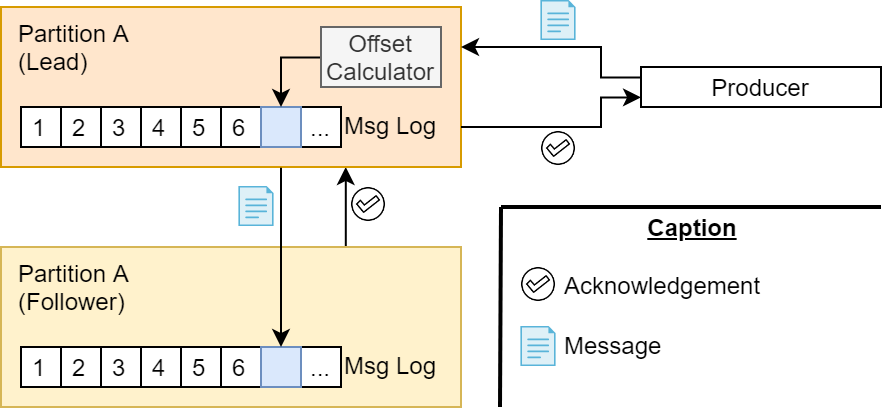
\includegraphics[width=\textwidth, height=0.9\textheight, keepaspectratio]{kafka_publish_message.png}
	\caption{Kafka publish message example}
	\label{img:kafkapubmsg}
\end{figure}

After explaining \textit{Kafka} and the concepts on which it is based, the open question arises as to what \textit{Kafka} is good for.
\textit{Kafka} can be used as a messaging system, which has already been described in the above communication example.
This includes the two traditional models of \textit{queue} and \textit{publish-subscribe}.
Queuing is realized by having multiple consumers within a consumer group.
Messages from a topic can only be consumed by one consumer within a consumer group.
There is an important side effect that the maximum number of consumers within a group is equal to the number of topic partitions.
On the other hand, \textit{publish-subscribe} is handled in such a way that several consumer groups can listen to the same topic.
In this way, each consumer group receives a published message.

Another specialty of \textit{Kafka} is its storage system.
Published messages are stored on disk, and Kafka’s disk structure enables good performance even when terabytes of data are stored.
The messages can be re-consumed as needed, making \textit{Kafka} a distributed file system for special purposes, designed for high performance, low-latency and replication.
The last feature of \textit{Kafka} is its ability to process data streams.
\textit{Kafka} provides a \textit{Streams API} that can consume and process messages from one topic and publish them to another topic.
This is very flexible because it uses the same interfaces as the actual producers and consumers \cite{ApacheKafka.01.06.2020}.

This concludes the general structure and major characteristics of \textit{Kafka}, but there are more features that are explained in \cite{Stopford.2018} and \cite{Kumar.2017}.
For example, an important feature that should be considered here is the message order guarantee.
\textit{Kafka}s default settings only guarantee message order within a partition.
It can be extended to guarantee the order within a topic or even globally, but this is associated with a high-performance overhead \cite[p.~30]{Kumar.2017}.
Another important fact is that \textit{Event Sourcing} architecture fits perfectly with \textit{Kafka}, since it can store messages like a database and replay the message log at any time.
Even if \textit{Kafka} is complex under the hood, it is still quite easy to use.
There are some quality of live features, such as not having to worry about queue depth and that slow consuming messages do not affect performance, which makes \textit{Kafka} easier the use.
\textit{Kafka}'s unique architecture allows for high speed reading of messaged.
Messages can be sent directly from storage because they are immutable logs.
As described at the beginning, \textit{Kafka} scales with virtually no limitations.
Finally, it offers countermeasures for denial of service attacks with a feature called \textit{quotas} \cite[p.~18ff.]{Stopford.2018}.
\label{cha:Technologies:communication:asynchronous}

\pagebreak
\section{Monitoring}\label{cha:Technologies:monitoring}
%!TEX root = ../../dokumentation.tex

In distributed systems, monitoring can be significantly more difficult than monitoring a monolithic architecture.
Metrics, like latency, traffic, errors and saturation as defined by the \textit{Google Site Reliability Engineering}, are essential from the DevOps perspective, but also for other business units.
In terms of microservices, monitoring makes necessary thresholds visible for scaling and can help to decide whether applications need to be broken down further and scaled individually.
Furthermore showing long term trends, retrospective analysis (e.g. for debugging) and especially alerting are core features of a monitoring system \cite{Ewaschuk.02.12.2019}.

\begin{figure}
	\centering
	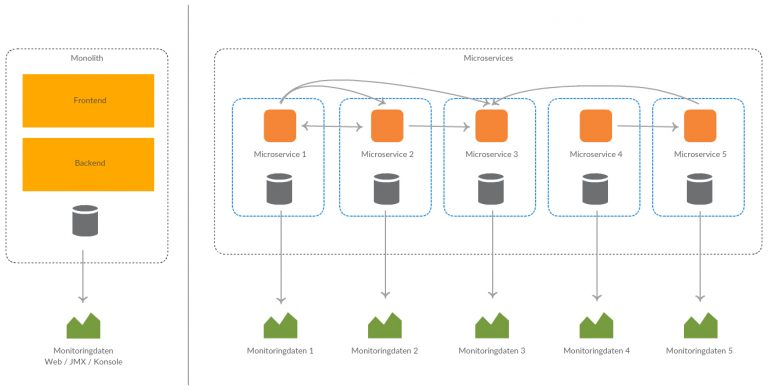
\includegraphics[width=\textwidth, height=0.9\textheight, keepaspectratio]{monitoringMonolithicComparison.jpg}
	\caption{Monolithic monitoring is easier to gather than with microservices~\cite{Fichtner.2016}}
	\label{img:monitoringMonolithicComparison}
\end{figure}

As opposed to a monolith, each microservice generates its own set of monitoring data, these have to be gathered and combined for a meaningful representation.
In order to pinpoint potential issues, metrics and logs from each service (depicted in Figure \ref{img:monitoringMonolithicComparison}) have to be centralized.
This aggregation can be done by either pushing or pulling.
Monitoring frameworks such as \textit{Prometheus} are pulling metrics from services, which have to implement an endpoint and serve data.
The implementation of a metrics endpoint is often called \textit{exporter}.
Time-series databases which do not primarily are built for monitoring (e.g. \textit{InfluxDB}, \textit{Graphite}) have to rely on data collection daemons, which are pushing data to the databases.
Popular daemons for example is the system-metric focused \textit{collectd} or the plugin-driven\textit{Telegraf}, with which a variety of services are supported at once \cite{Fichtner.2016}\cite{Richardson.20.05.2020}\cite{Ewaschuk.02.12.2019}.

In general, aforementioned metric collection daemons are inter-compatible.
Although \textit{Telegraf} would work best with \textit{InfluxDB}\footnote{Referring to the \textit{TICK} stack for centralized alerting and monitoring from the same company \textit{influxdata}: \textit{Telegraf}, \textit{InfluxDB}, \textit{Chronograf} (visualization) and \textit{Kapacitor} (data streaming engine)}, the metric output can be directed to other time-series databases like \textit{Graphite} and even replace the data ingest for \textit{Prometheus} \cite{Loschwitz.2018}.

For this work, the focus is on the time series database itself, as the data aggregation can be interchanged and are mostly compatible to one another.
Furthermore external visualizations such as \textit{Grafana} or \textit{Chronograf} are left out.

\begin{figure}
	\centering
	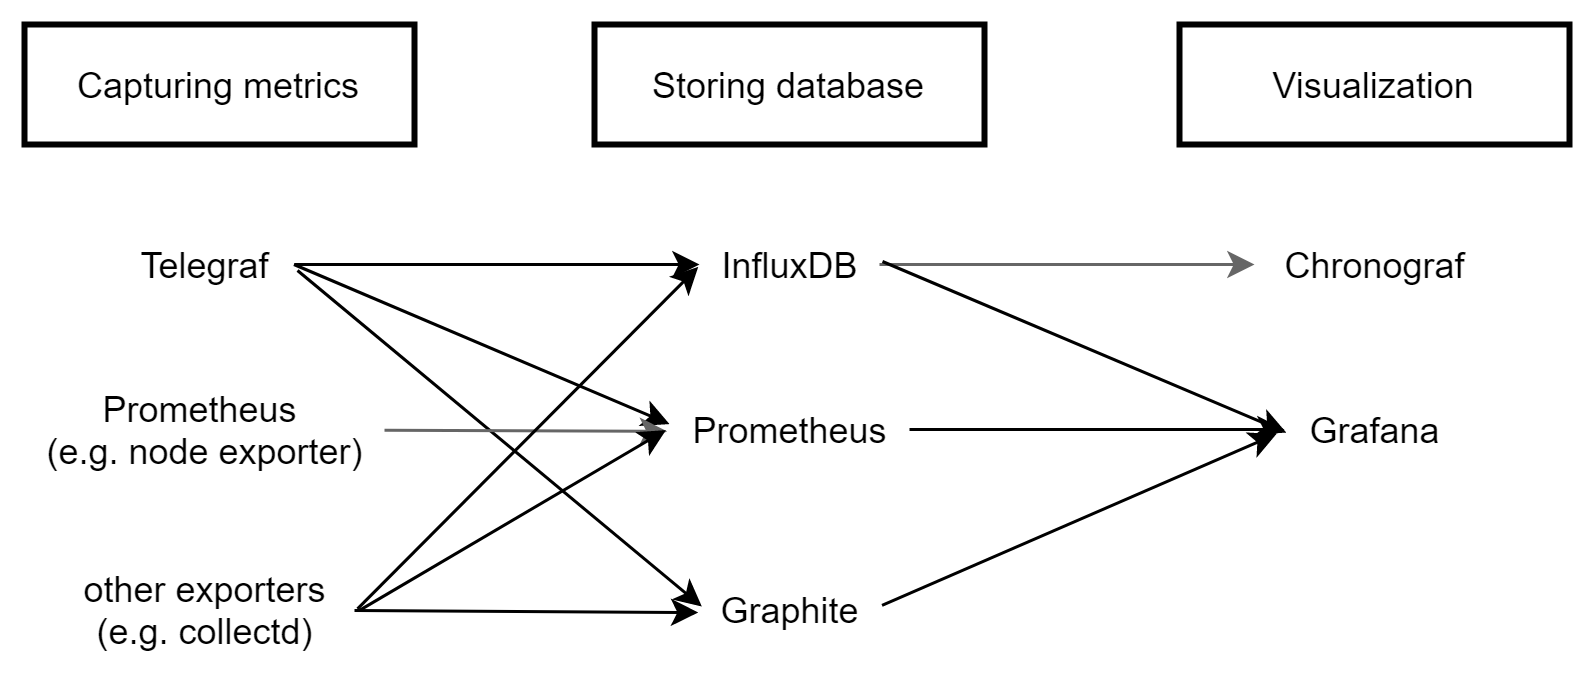
\includegraphics[width=\textwidth, height=0.9\textheight, keepaspectratio]{overviewmonitoring.png}
	\caption{Overview of an selection of popular monitoring technologies}
	\label{img:overviewmonitoring}
\end{figure}

\subsection{Graphite}

As a real-time graphing system based on Python, \textit{Graphite} is able to store numeric time-series data and render graphs.
In order to do so it consists of three main components, as shown in Figure \ref{img:overviewgraphite}, namely the daemon \textit{carbon}, the database library \textit{whisper} and the \textit{graphite webapp} for visualization \cite{Davis.08.05.2020b}.
Unlike \textit{Prometheus} for instance, it relies on inbound metric submissions and does not collect data actively.
Consequently, applications or nodes to be monitored have to be equipped with collection tools, which either communicate over TCP or UDP as plain text, using Python's \textit{pickle} protocol or \ac{AMQP} \cite[p.~49]{Dixon.2017}\cite{Davis.08.05.2020c}.

In most cases, however, tools already support the format, as seen in Listing \ref{listing:graphitemessage}, and handle metrics export and communication with \textit{Graphite}'s \textit{carbon-cache}.
An extensive list of currently supported collectors as well as further compatible tools, which should be used in conjunction, can be found in the \textit{Graphite} documentation \cite{Davis.08.05.2020d}.

\begin{lstlisting}[caption=Graphite Message Format, label=listing:graphitemessage]
metric_path value timestamp
\end{lstlisting}

\begin{lstlisting}[caption=Graphite's dot oriented naming scheme, label=listing:graphitemetricnaming]
api_server_http_requests_total.post.500.tracks.sample1 
\end{lstlisting}

The logical component \textit{carbon} as shown in Figure \ref{img:overviewgraphite} consists of a relay, an aggregator and the actual required \textit{carbon-cache}.
The latter represents the core to accept metrics over aforementioned protocols.
A \textit{Graphite} message (if not bundled using Python's \textit{pickle}) contains the metric namespace to be populated (\textit{metric\_path}), the \textit{value} and a timestamp, as seen in Listing \ref{listing:graphitemessage} \cite{Davis.08.05.2020c}.
\textit{Graphite}'s metrics naming is dot oriented and implies hierarchy.
In Listing \ref{listing:graphitemetricnaming} an exemplary metric name is given for HTTP POST requests with the \textit{response code 500} landing on the \textit{/tracks} endpoint.

\begin{figure}
	\centering
	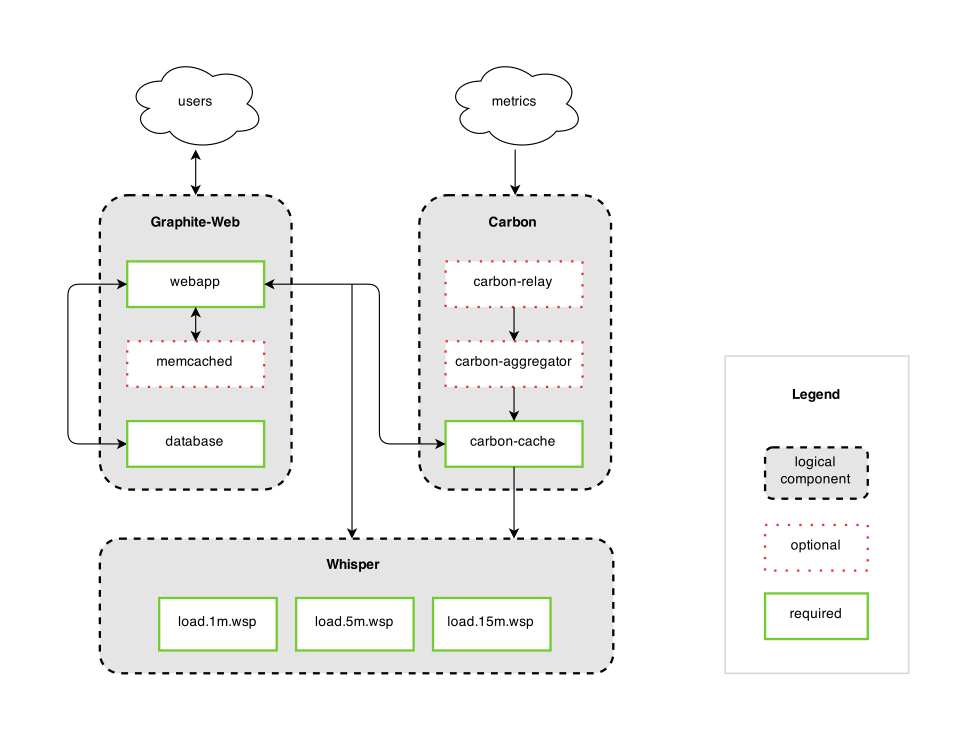
\includegraphics[width=\textwidth, height=0.8\textheight, keepaspectratio]{graphiteoverview.png}
	\caption{Overview of Graphite's architecture \cite{Davis.08.05.2020}}
	\label{img:overviewgraphite}
\end{figure}

The relay is needed for scaling the \textit{carbon-cache} processes, which can be on different servers.
However, in practice typical load balancers such as \textit{HAProxy} are used in front of the logical component \textit{carbon} as a whole to split metrics and thus scaling \textit{Graphite} \cite{Dubiel.29.05.2020}.
In order to reduce load, an aggregator can be used to buffer metrics before saving them using \textit{whisper}, which is a fixed sized database file format for datapoints \cite[p.~52]{Dixon.2017}.
Each \textit{*.wsp} file in\textit{whisper} needs corresponding scheme definitions for retention policies and precision settings.
These settings can be used to duplicate metrics with a lower precision to save space, while removing the original after its retention duration \cite[p.~55]{Dixon.2017}.
Lastly \textit{graphite-web} can be used to visualize data in real-time from the \textit{whisper} storage and \textit{carbon-cache} simultaneously.


The performance of \textit{Graphite} is generally bound to the \ac{I/O} performance of the system.
Usually this is mitigated by increasing the disk array, placing aggregators and load balance between them.
Although this way of vertical scaling is supported well, horizontal scaling can be cumbersome, as one has to decide between redundancy (replication factor) or high performance by utilizing consistent hashing across all instances \cite[p.~57ff.]{Dixon.2017}.
Possible currently used and common alternatives to avoid the scaling problem, are replacing the underlying \textit{whisper} storage engine (e.g. with \textit{InfluxDB}) or replacing the relay with alternative implementations (e.g. \textit{carbon-relay-ng} written in Go) to achieve higher performance.

\subsection{InfluxDB}

\textit{InfluxDB} is a time series database and provides an SQL-like query language (\textit{InfluxQL}) for data interaction, unlike \textit{Graphite}.
The company \textit{influxdata}, provides an open-source version (\textit{InfluxDB OSS}) and a commercial version (\textit{InfluxDB Enterprise}).
Although \textit{InfluxDB} has a higher performance than \textit{Graphite}, as shown in an extensive technical paper, including benchmarks, and thus would be a very good database for monitoring usages, it can not be taken into consideration due to missing features \cite{influxdata.2019}.
The main reason is the missing clustering option for the database.
In the open-source variant, high availability is not guaranteed and horizontal scalability through sharding is not available.
Especially when deploying a high demanding application, such as a large management application, operating \textit{InfluxDB} on a single node seems to be insufficient \cite{influxdata.2020}.
Consequently, no overview will be given here as non open-source and especially paid features are not in the scope of research, leaving \textit{InfluxDB OSS} not suitable.

\subsection{Prometheus}

Similar to \textit{Graphite}, \textit{Prometheus} is primarily used for system monitoring and includes a time-series database and a monitoring system.
Currently \textit{Prometheus} is part of the \textit{Cloud Native Computing Foundation} and open source.
Besides storing and retrieving metrics, it also includes an alerting system and a web \ac{UI}.
Moreover, \textit{Prometheus} has a broad support of clients, by using exporters on the client side.
Unlike other monitoring solutions which depend on passive listeners and clients pushing metrics to the service, \textit{Prometheus} mainly relies on pulling \cite{Berman.2018}\cite{PrometheusAuthors.30.05.2020}.

\begin{figure}
	\centering
	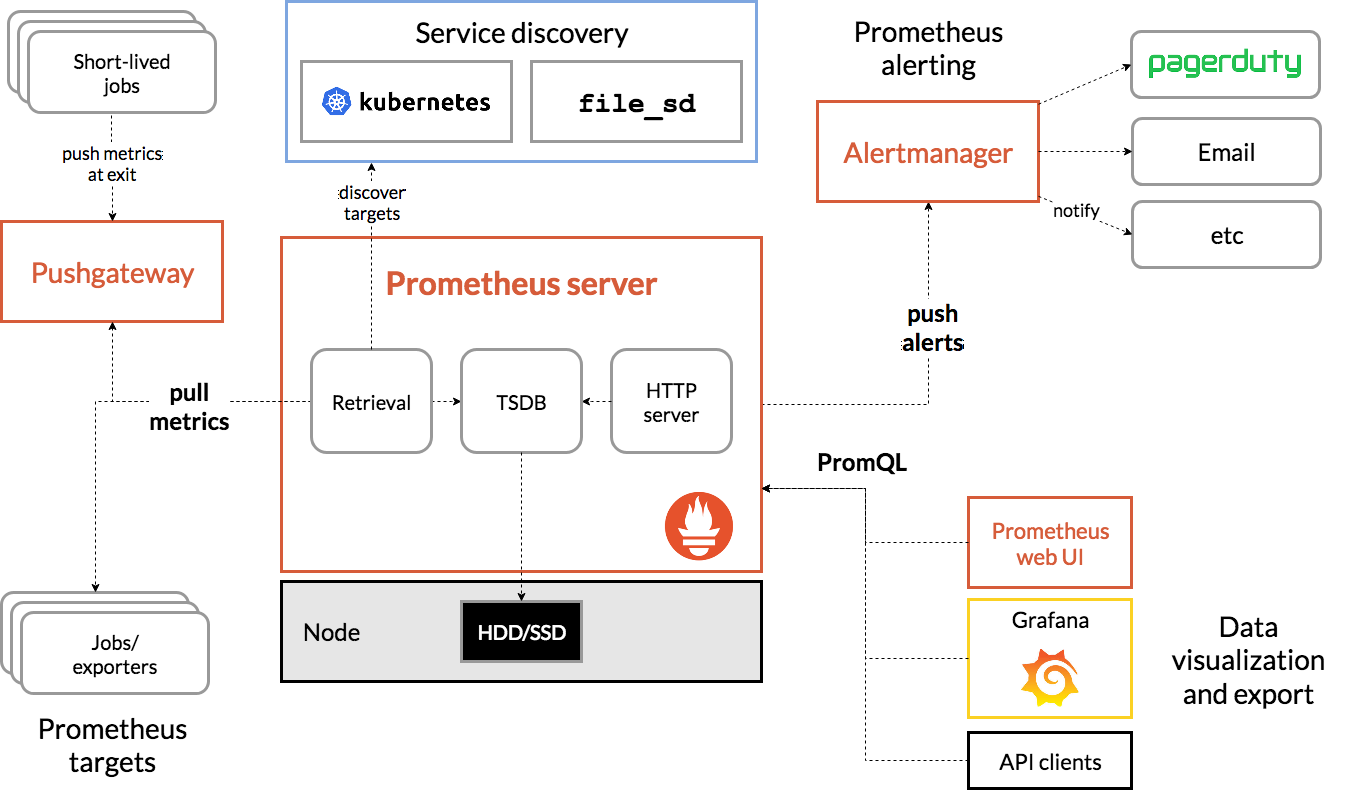
\includegraphics[width=\textwidth, height=0.8\textheight, keepaspectratio]{prometheusoverview.png}
	\caption{Overview of Prometheus' architecture \cite{PrometheusAuthors.30.05.2020}}
	\label{img:prometheusoverview}
\end{figure}

As seen in Figure \ref{img:prometheusoverview} metrics are pulled from \textit{Prometheus} target, which expose their metric on a \ac{HTTP} endpoint.
Consequently, \textit{Prometheus} handles data scraping itself and stores it in an internal \ac{TSDB}.
Although the concept of pulling is favored, \textit{Prometheus} is compatible with existing \enquote{pushing} clients as well, by utilizing the intermediary \textit{Pushgateway}, which stores and aggregates data.
For the active pulling, the endpoints can either be static, or be discovered by utilizing external service registries.
Apart from collecting and storing metrics, events and alerts can be configured in the \textit{Alertmanager} for sending notifications.
Lastly, external visualizations and clients can communicate with \textit{Prometheus} using its own \textit{Prometheus Query Language (PromQL)} \cite{PrometheusAuthors.30.05.2020}.

Similarly to \textit{Graphite}'s \textit{whisper}, time series are stored locally and are grouped into blocks.
With \textit{Prometheus}, incoming samples are kept in memory first and are secured with a write-ahead-log, before being persisted and grouped into two hour blocks.
Like \textit{Graphite}, retention policies and compression options are available for the \ac{TSDB} format.
This approach however, can limit the scalability and durability of the system, as the local storage is bound to the performance of a single node, especially with the concept of node autonomy found in \textit{Prometheus}.
Possible solutions are to replace the \ac{TSDB}, against remote storage systems, to which \textit{Prometheus} communicates with protocol buffers over \ac{HTTP} \cite{PrometheusAuthors.30.05.2020b}.

\textit{Prometheus} is generally known for the variety of exporters available for \acp{API}, messaging systems, hardware related metric systems and also databases. (see \cite{PrometheusAuthors.30.05.2020c} for an extensive list)
Instead of converting existing metrics to the \textit{Prometheus} exposition format, using aforementioned exporters, client libraries are available as well, with which metrics of an application are defined and exposed.

Similar to the \textit{Graphite} message format (see Listing \ref{listing:graphitemessage}), one can also write raw messages, which include the metric name, value and timestamp \cite{PrometheusAuthors.30.05.2020d}.
However, the data model of \textit{Prometheus} allows more complex metadata models by including \enquote{labels}, i.e. key values pairs.
Depicted in Listing \ref{listing:prometheusmessage} is an exemplary metric of the number of HTTP POST requests with the \textit{response code 500} to the \textit{/tracks} endpoint.
This explicit multidimensionality allows greater flexibility compared to the implicit dimension encoding found in \textit{Graphite}, which makes progressive changes in naming difficult to maintain (compare Listings \ref{listing:graphitemetricnaming} and \ref{listing:prometheusmessage}) \cite{Berman.2018}\cite{PrometheusAuthors.30.05.2020e}.

\begin{lstlisting}[caption=Prometheus exposition format with example, label=listing:prometheusmessage]
// syntax: metric_name{label_name = label_value, ...} value [timestamp]

api_server_http_requests_total{method="POST",handler="/tracks",status="500"} 34
\end{lstlisting}

With the aforementioned concept of write ahead logs for instance, reliability is one of the core principles.
The autonomy of each \textit{Prometheus} instance allows access to metrics, even under failure conditions.
However, just like \textit{Graphite}, scaling may be difficult.
A common approach is splitting up the metrics to be monitored and the \textit{Prometheus} instance bound to it, which would value the autonomy aspect.
Alternatively \textit{Prometheus} can scale horizontally by sharding , which means that a subset of metrics are scraped by slaves (partitioning) and are then federated by the master \cite{Brazil.2015}\cite{Berman.2018}.

\pagebreak
\section{Selection}\label{cha:Technologies:selection}
%!TEX root = ../../dokumentation.tex

\subsection{Synchronous Communication}\label{cha:Technologies:selection:synchronous}

When comparing the three presented synchronous messaging technology, \textit{gRPC} is the most performant, thus fulfilling the requirements of the user and developer (cf. chapter \ref{cha:Requirement:persona}) the most.
Its binary format (\textit{protocol buffer}), as opposed to \ac{JSON} used in \textit{GraphQL} and \ac{REST}, is more efficient and beneficial in cases with low network throughput or limited resources.
However, due to missing official support of \textit{gRPC-Web} and due to its incomplete implementation, communication between the web-based frontend and any backend can only be achieved with \ac{REST} and \textit{GraphQL}.
Consequently \textit{gRPC} could only be used for backend communication in this use case.

\begin{table}[h!]
	\begin{tabularx}{\linewidth}{ |l| X | X | X | }
		\hline
		&
		RESTful HTTP & GraphQL                                                                   & gRPC                                                                                                                                                                      \\
		\hline
		Protocols   & Synchronous communication over HTTP only                                  & Synchronous or asynchronous in multiple protocols (e.g. HTTP, AMQP, MQTT)           & Synchronous communication in HTTP2 (although asynchronous implementation available) \\
		Design      & HTTP (verbs, links, status codes)                                         & Based on exchanging messages                                                        & Messages (e.g. protocol buffer payload)                                             \\
		Standards   & Multiple standards available (e.g. Richardson Maturity Model, OpenAPI)    & Schema definition as a standard (\ac{IDL}) Strongly typed                           & Service definition in protocol buffer file for instance (strongly typed as well)    \\
		Payload     & \ac{JSON} for instance                                                    & \ac{JSON}                                                                           & Serialized in binary(default is protocol buffer)                                    \\
		Integration & Nearly every client                                                       & Specific implementation in clients needed (wrapping in \ac{HTTP} endpoint possible) & Specific and tightly coupled implementation for clients needed                      \\
		Endpoint    & Endpoints need to be known, hypermedia possible with HATEOAS for instance & Single endpoint, self-describing scheme                                             & Concrete methods have to exist on both sides                                        \\
		Scaling     & Easy to scale due to stateless nature                                     & Scaling only limited by data source access bottlenecks                              & Scaling similar to REST as HTTP2 is used                                            \\
		\hline
	\end{tabularx}
	\caption{Overview synchronous communication \cite{Rocha.2019}}
	\label{tab:overviewSynchronousCommunication}
\end{table}

Regarding the scalability of the application, all three technologies excel and provide high performance endpoint access.
Load balancing is possible with all three of them with \textit{gRPC} being the most advanced due to HTTP2.
Another aspect is the ease of use and the maintainability of the protocol.
Contrary to the loosely specified \ac{REST}, both \textit{GraphQL} and \textit{gRPC} provide strong typing by enforcing schema/service definitions.
This makes validation and error handling easier for both sides.
Although having specified schemes, \textit{GraphQL} is the most flexible compared to \textit{gRPC}, due to its nature being an \ac{RPC} framework.
With \textit{gRPC}, concrete methods and response actions have to be implemented, while also having to update the client when changes occur.
Consequently \textit{gRPC} introduces tight coupling between services.
On the other side is \textit{GraphQL} with a flexible requests and an introspective, self-describing single endpoint.
\ac{REST}, however fares worse in comparison, as there are no endpoint specifications per default and issues such as over- and underfetching may occur.

Tight coupling in a microservice may not be necessarily bad practice, as it can bring benefits in a tightly coupled network of services, such as low latency and high efficiency found in \textit{gRPC} \cite{Esposito.2019}.
However, in the case of the exemplary use case in this work, loose coupling is better with a modular approach for adding new components to the application.
This renders \textit{gRPC} with its coupling by design disadvantageous, compared to \textit{GraphQL} and \ac{REST}.

In conclusion, \textit{gRPC} represents a highly efficient but tightly coupled system, whereas \textit{GraphQL} allows flexible and maintainable data queries and RESTful \ac{HTTP} being a widespread used, but less standardized and possibly less efficient way of messaging.
An overview is given in the Table \ref{tab:overviewSynchronousCommunication}.

Albeit \textit{gRPC} being developed out of the need for performant and low latency microservice communication, the support for the component in the architecture with the most intensive synchronous communication, namely frontend to backend is incomplete \cite{gRPCAuthors.01.06.2020}.
Regarding inter-service communication, in which \textit{gRPC} dominates and \textit{GraphQL} on the other hand is unsuited, broker-based communication may be preferable.
This is due to the fact that the different components are emitting events affecting multiple other components, instead of just having to trigger a function with a point to point connection like with \ac{RPC} (e.g. ending a match affects both the component \textit{Scoreboard} and \textit{Events}, cf. chapter \ref{cha:Requirement:lanpartyapplication}).
All things considered \ac{REST} and \textit{GraphQL} are prototyped and evaluated in this work, although \textit{gRPC} might be an option to be considered in the future for this use case, with coming web application support.


\pagebreak

\subsection{Asynchronous Communication}\label{cha:Technologies:selection:asynchronous}

If one compares the three asynchronous messaging technologies presented, \ac{NATS} is the most performant and thus meets the requirements of the personas (cf. chapter \ref{cha:Requirement:persona}) the most.
In a benchmark comparison between \ac{NATS} Streaming and \textit{Apache Kafka}, \ac{NATS} Streaming was faster in almost all tests \cite{TylerTreat.2016}.
However, this performance has its price, as \ac{NATS} does not persist messages.
Therefore, they are lost if no consumer listens for them.
On the other hand, \textit{RabbitMQ} provides mechanisms to route messages that are not read, and \textit{Apache Kafka} stores the messages, which eliminates the problem altogether.

\begin{table}[h!]
	\begin{tabularx}{\linewidth}{ |l| X | X | X | }
		\hline                                                                                            &   
		RabbitMQ                                                                                          &   
		NATS                                                                                              &   
		Apache Kafka                                                                                        \\
																
		\hline
		Protocol                                                                                          &   
		\ac{AMQP}, \ac{MQTT} and \ac{STOMP}                                                               &   
		NATS                                                                                              &   
		Kafka                                                                                               \\
																
		Communication                                                                                     &   
		Publish-Subscribe and Queue                                                                       &   
		Publish-Subscribe, Queue and Request-Response                                                     &   
		Publish-Subscribe, Queue and Streaming                                                              \\
																
		Payload                                                                                           &   
		\ac{AMQP} and \ac{MQTT} is binary and \ac{STOMP} is plain text                                    &   
		plain text                                                                                        &   
		developer can choose \cite{RobinMoffatt.2018}                                                          \\
																
		Quality of Service                                                                                &   
		\textit{at-most-once}, \textit{at-least-once} and \textit{exactly once} \cite{PaoloPatierno.2018} &   
		\textit{at-most-once} and \textit{at-least-once} (if \textit{NATS Streaming} is used)             &   
		\textit{at-most-once} and \textit{at-least-once} \cite{AjmalKaruthakantakath.2016}                  \\
		Queue Storage                                                                                     &   
		Limited                                                                                           &   
		None                                                                                              &   
		Permanent                                                                                           \\
		\hline
	\end{tabularx}
	\caption{Overview asynchronous communication}
	\label{tab:overviewAsynchronousCommunication}
\end{table}

All three technologies provide a sophisticated scaling solution that enables high availability.
Another aspect is usability, which is difficult to measure because it is subjective.
To simplify this, only the complexity of available commands is used as a measurement.
This leaves \textit{RabbitMQ} with the \ac{AMQP} protocol behind \ac{NATS} and \textit{Apache Kafka}, because connecting to a queue or exchange requires extensive configuration.
On the other hand, \ac{NATS} and \textit{Apache Kafka} strive for a simple interface \cite[p.~8]{Quevedo.2018} \cite[p.~18]{Stopford.2018}.
However, \textit{RabbitMQ} also supports \ac{MQTT} and \ac{STOMP} via plugin, which simplifies the necessary configuration.
It is important to note that simplicity does not mean that only simple structures are possible.
As far as resilience is concerned, each technology has its own clues to ensure it.
Interesting features include \textit{Apache Kafka} \textit{quotas} \cite[p.~21]{Stopford.2018} and the fact that \ac{NATS} will break connections if the consumer becomes too slow \cite[p.~9]{Quevedo.2018}.

From the persona perspective, \ac{NATS} and \textit{Apache Kafka} would be selected, but it is also important that the technologies fits the exemplary use case in this work.
The components of the use case were presented in the requirement analysis (cf. chapter \ref{cha:Requirement:lanpartyapplication}).
The communication between them is the important aspect when choosing an asynchronous messaging technology.
There is no obvious communication scenario in which extreme performance would be required.
Even if, for example, the \textit{billing} component takes 10 seconds to communicate with the \textit{event} component, no problem should occur.
Therefore, the components should work independently of each other, and eventual consistency is acceptable if the communication provides the \ac{QoS} \textit{at-least-once}.

In summary, \textit{RabbitMQ} and \textit{Apache Kafka} meet the requirements "out of the box", and if \textit{NATS Streaming} is used instead of \ac{NATS}, all three technologies can be used.
However, selection is required, so \ac{NATS} is not selected because it does not provide the required functionality out of the box.

\subsection{Monitoring}\label{cha:Technologies:selection:monitoring}

Regarding the monitoring of a microservice environment, important aspects are the performance, ease of use and the resilience of the system. (cf. chapter \ref{cha:Requirement:persona})
Another aspect is the scalability, which, due to the limited options of horizontal scaling for both options, is neglected here.
Both technologies do allow scaling via sharding and/or federation mechanisms, which, however, creates disadvantageous coupling.

The ease of use overall is greater with \textit{Prometheus}  than with \textit{Graphite} , due to the larger compatibility with various client services.
It should be noted however, that the initial setup and metric pushing is easier with \textit{Graphite}  due to the raw communication protocols.
Especially with simpler services to be monitored, or short running jobs, avoiding heavy \ac{HTTP} handling is favorable.
Moreover the push based metric collection in \textit{Graphite}, allows it to be flexible, as it does not need a service discovery, which \textit{Prometheus}  needs to avoid static endpoint links \cite{Erez.2019}.


However, the relatively more complicated manual integration of instrumentation libraries in order to export metrics in the \textit{Prometheus}  message format, can be neglected, as third-party exporters are available.
This extensibility with metric exporters, which allow very easy integration of services, make \textit{Prometheus}  more favorable in a possibly highly diverse and polyglot microservice environment.
Although this does cause additional dependencies and requires \textit{Prometheus}  to
run inside the same network, due to the pull strategy unlike \textit{Graphite} , the higher performance of \textit{Prometheus}  is overweighing.
\textit{Graphite} 's ingestion process for example be overwhelmed, when sending a lot of datapoints, rendering the pushing concept disadvantageous \cite{Erez.2019}\cite{Frazier.2019}.

\begin{table}[h!]
	\begin{tabularx}{\linewidth}{ | l | X | X | }
		\hline
		Feature                 & Prometheus                                                           & Graphite                                                       \\
		\hline
		Metric input            & Server scrapes/pulls metrics from clients                            & Metrics are pushed to Graphite                                 \\
		Communication protocols & HTTP-based endpoint                                                  & TCP, UDP, AMQP                                                 \\
		Metric discovery        & Service discovery with Kubernetes for instance                       & no client discovery                                            \\
		Metric naming scheme    & Naming system using labels (key-value)                               & Hierarchical dot notation                                      \\
		Data operations         & Prometheus Query Language \textit{PromQL}                            & Graphite Functions                                             \\
		Client support          & More complicated initial setup, but many exporters available already & Simple metric export, but fewer support. Custom scripts needed \\
		\hline
	\end{tabularx}
	\caption{Comparison monitoring Graphite and Prometheus \cite{Erez.2019}\cite{Frazier.2019}\cite{Berman.2018}}
	\label{tab:comparisonmonitoring}
\end{table}

When comparing the resilience, \textit{Graphite} 's push strategy forces clients having to update the endpoint, when changes occur to the monitoring system, making a failover less flexible.
While \textit{Graphite}  does support external storage clusters and thus provide redundancy, autonomous \textit{Prometheus}  instances do not support any type of redundancy when a cluster fails, as any metric requests have to pass through \textit{Prometheus} , regardless of the data source.
On the other hand, \textit{Prometheus}  provides inbuilt monitoring of containers, essential to microservices.
Moreover, \textit{Prometheus}  is able to monitor uptime through the metric scraping/pulling process \cite{Berman.2018}\cite{Erez.2019}.

To conclude, \textit{Prometheus}  has various benefits such as an ecosystem of exporters and client instrumentation, which reduces the more complex nature of \textit{Prometheus} .
On the contrary, \textit{Graphite}  has a simpler format and communication structure, partly due to the incorporated push strategy.
A brief comparison overview can also be found in Table \ref{tab:comparisonmonitoring}.
For the microservice architecture to be built in this work, \textit{Prometheus}  is chosen, due to the integration capabilities with other services through modular exporters, the service discovery capabilities and the higher performance.
The aforementioned traits are essential in an application like a \ac{LAN} party management tool, where high user interaction with a diverse backend occurs.
Additionally there are other topics of \textit{Prometheus} , which are not covered here, but are important for this specific use case, namely event tracking, alarming and the extensive query language \textit{PromQL}.

A prototypic implementation for both technologies, however, is left out in the following, as monitoring is highly variable regarding the architecture.
Each monitoring solution might work better, depending on the metrics to be monitored and the used technologies.
As each technology has different metric reporting solutions for delivering or exporting data to corresponding monitoring technologies, an evaluation whether \textit{Graphite}  or \textit{Prometheus}  would work best, can only be done after selecting other components in a microservice environment.
The communication technology and services for the exemplary application however, still have to be evaluated with prototypes.
Consequently the choice for \textit{Prometheus}  made here should be considered with caution, and may not be applicable to every microservice environment.
